\documentclass{../../slides-style}

\slidetitleext{Лекция 10: Тестирование и дефекты}{25.04.2023}{Тестирование и дефекты}

\begin{document}

    \begin{frame}[plain]
        \titlepage
    \end{frame}

    \section{Тестирование}

    \begin{frame}
        \frametitle{Тестирование}
        \begin{itemize}
            \item Любая программа содержит ошибки
            \item Если программа не содержит ошибок, их содержит алгоритм, который реализует эта программа
            \item Если ни программа, ни алгоритм ошибок не содержат, такая программа даром никому не нужна
        \end{itemize}
    \end{frame}

    \begin{frame}
        \frametitle{Ошибки}
        \begin{itemize}
            \item Не несоответствие техническому заданию, а несоответствие ожиданиям
            \item Процесс тестирования субъективен
        \end{itemize}
    \end{frame}

    \begin{frame}
        \frametitle{Баг}
        \begin{center}
            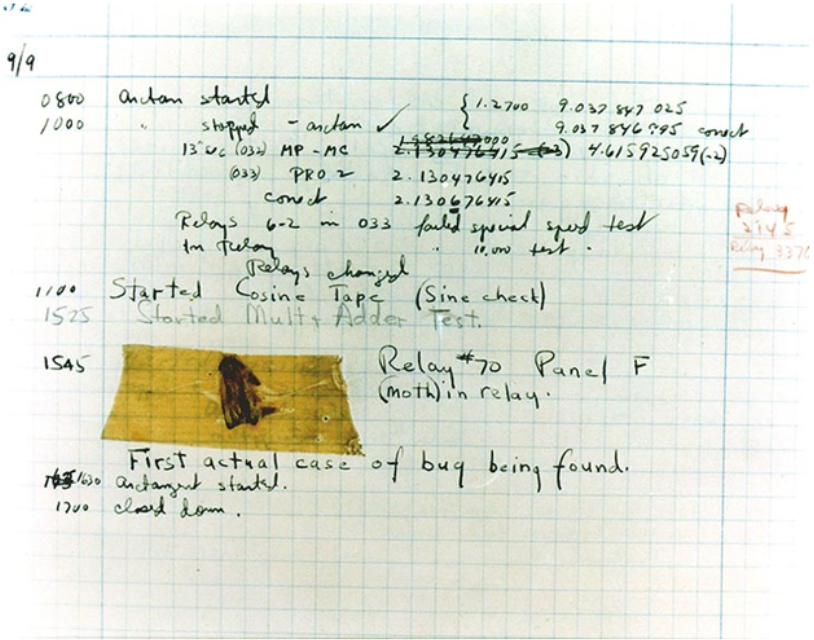
\includegraphics[width=0.7\textwidth]{bug.png}
            \attribution{https://education.nationalgeographic.org/resource/worlds-first-computer-bug/}
        \end{center}
    \end{frame}

    \begin{frame}
        \frametitle{Цель тестирования}
        \begin{itemize}
            \item Тестирование --- процесс поиска ошибок
            \begin{itemize}
                \item Тест, не выявивший ошибку --- впустую потраченное время
                \begin{itemize}
                    \item Не совсем правда, есть регрессионные тесты
                \end{itemize}
            \end{itemize}
            \item Тестирование не может доказать, что ошибок в программе нет
            \begin{itemize}
                \item Субъективность ошибок
                \item Огромное количество входных данных
                \begin{itemize}
                    \item Программа, складывающая два целых числа --- сотни лет на полный тест
                \end{itemize}
                \item Огромное количество путей исполнения
                \begin{itemize}
                    \item 1979 год, около 20 строк кода, сто триллионов путей исполнений
                \end{itemize}
            \end{itemize}
            \item Формальная верификация
        \end{itemize}
    \end{frame}

    \begin{frame}
        \frametitle{Виды тестирования}
        \framesubtitle{Классификация по тому, что тестируется}
        \begin{itemize}
            \item Функциональное тестирование
            \item Тестирование производительности
            \begin{itemize}
                \item Нагрузочное
                \item Стресс-тестирование
                \item Тестирование стабильности
                \item Тестирование конфигурации
            \end{itemize}
            \item Тестирование пользовательского интерфейса
            \item Тестирование удобства использования
            \item Тестирование безопасности
            \item Тестирование локализации
            \item Тестирование совместимости
        \end{itemize}
    \end{frame}

    \begin{frame}
        \frametitle{Виды тестирования}
        \framesubtitle{Классификация по масштабности тестирования}
        \begin{columns}
            \begin{column}{0.4\textwidth}
                \begin{itemize}
                    \item Модульное
                    \item Интеграционное
                    \item Системное
                    \begin{itemize}
                        \item В т.ч. тестирование пользовательского интерфейса
                    \end{itemize}
                \end{itemize}
            \end{column}
            \begin{column}{0.6\textwidth}
                \begin{center}
                    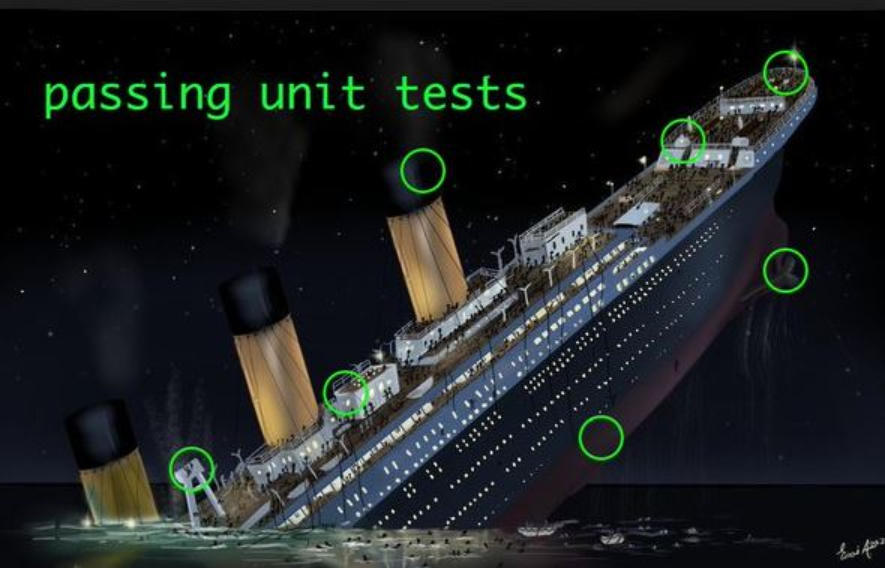
\includegraphics[width=\textwidth]{titanic.png}
                \end{center}
            \end{column}
        \end{columns}
    \end{frame}

    \begin{frame}
        \frametitle{Виды тестирования}
        \framesubtitle{По этапу жизненного цикла}
        \begin{itemize}
            \item Смоук-тестирование
            \item Регрессионное тестирование
            \item Альфа-тестирование
            \item Бета-тестирование
            \item Релиз-кандидат
        \end{itemize}
    \end{frame}

    \begin{frame}
        \frametitle{Виды тестирования}
        \framesubtitle{По знанию о системе}
        \begin{itemize}
            \item Тестирование <<чёрного ящика>>
            \item Тестирование <<белого ящика>>
            \item Тестирование <<серого ящика>>
            \item Исследовательское тестирование
        \end{itemize}
    \end{frame}

    \section{Тестирование и жизненный цикл}

    \subsection{Тестирование требований}

    \begin{frame}
        \frametitle{Тестирование требований}
        \begin{itemize}
            \item Однозначность
            \begin{itemize}
                \item слова <<обычно>>, <<как правило>>, <<иногда>>, <<необязательно>> и т.п.
                \item субъективные оценочные суждения: <<удобно>>, <<быстро>>, <<гибко>> и т.п.
            \end{itemize}
            \item Атомарность (без предлогов и/или)
            \item Чёткий критерий приёмки (acceptance criteria)
            \item Отсутствие избыточных и противоречивых требований
            \item Мотивация каждой роли
            \item Не предполагает конкретного способа реализации
        \end{itemize}
    \end{frame}

    \begin{frame}
        \frametitle{Критерии INVEST}
        \begin{itemize}
            \item I --- Independent, независимое от остальных
            \item N --- Negotiable, то есть его можно обсудить и изменить
            \item V --- Valuable, имеющее ценность для пользователя
            \item E --- Estimable, трудоёмкость его реализации можно оценить
            \item S --- Small, его можно реализовать в разумные сроки (один спринт или одну итерацию разработки)
            \item T --- Testable, можно протестировать его выполнение
        \end{itemize}
    \end{frame}

    \begin{frame}
        \frametitle{Критерии приёмки}
        \begin{itemize}
            \item Чёткие
            \item Контекст-действие
            \item Однозначно документирующие поведение системы
            \item Добросовестные
        \end{itemize}
    \end{frame}

    \subsection{Тестирование архитектуры}

    \begin{frame}
        \frametitle{Тестирование архитектуры}
        \begin{itemize}
            \item Аккуратность декомпозиции
            \begin{itemize}
                \item Dependency Inversion
                \item Слои
                \item Микросервисы
                \begin{itemize}
                    \item Опасайтесь <<микросервисного монолита>>
                \end{itemize}
            \end{itemize}
            \item Простота
            \item Наблюдаемость
            \begin{itemize}
                \item Возможность развернуть окружение
                \item Быстрая обратная связь
                \item Логирование
                \begin{itemize}
                    \item Поддержанное инструментами, например ElasticSearch и Kibana
                \end{itemize}
                \item Трассируемость
                \item Метрики
            \end{itemize}
        \end{itemize}
    \end{frame}

    \subsection{Тестирование и реализация}

    \begin{frame}
        \frametitle{Пирамида тестирования}
        \begin{center}
            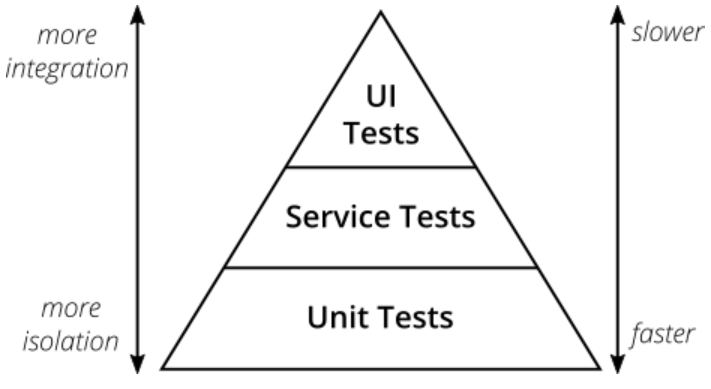
\includegraphics[width=0.7\textwidth]{testPyramid.png}
            \attribution{https://martinfowler.com/articles/practical-test-pyramid.html}
        \end{center}
    \end{frame}

    \begin{frame}
        \frametitle{Тестовые сценарии, свойства}
        \begin{itemize}
            \item Идентификатор и название
            \item Предварительные шаги
            \item Тестовые шаги
            \begin{itemize}
                \item Действие --- ожидаемый результат
            \end{itemize} 
            \item Итоговый ожидаемый результат
            \item Шаги по восстановлению окружения
            \item Конфигурация
            \item Тэги
            \item Зависимости
        \end{itemize}
    \end{frame}

    \begin{frame}
        \frametitle{Тесты, терминология}
        \begin{itemize}
            \item Сьюты
            \item Проекты
            \item Тестовые прогоны
            \begin{itemize}
                \item Статус
                \item Результаты по каждому шагу
            \end{itemize}
            \item Тест-планы
            \begin{itemize}
                \item Отобранные тестовые сценарии
                \item Календарные сроки
                \item Ответственные
            \end{itemize}
        \end{itemize}
    \end{frame}

    \begin{frame}
        \frametitle{Пример тестового сценария}
        \begin{center}
            \begin{tabu} {| X[0.6 l p] | X[1 l p] |}
                \tabucline-
                \everyrow{\tabucline-}
                \textbf{Что делаем}                             & \textbf{Что происходит}                                                            \\
                Вводим \textit{adder} и жмём на \textit{Enter}  & Экран мигает, внизу появляется знак вопроса                                        \\
                Нажимаем 2                                      & За знаком вопроса появляется цифра 2                                               \\
                Нажимаем \textit{Enter}                         & В следующей строке появляется знак вопроса                                         \\
                Нажимаем 3                                      & За вторым знаком вопроса появляется цифра 3                                        \\
                Нажимаем \textit{Enter}                         & В третьей строке появляется 5, несколькими строками ниже --- ещё один знак вопроса
            \end{tabu}
        \end{center}
    \end{frame}

    \begin{frame}
        \frametitle{Выявленные проблемы}
        \begin{itemize}
            \item Нет названия программы на экране, может, мы запустили не то
            \item Нет никаких инструкций, пользователь без идей, что делать
            \item Непонятно, как выйти
        \end{itemize}
    \end{frame}

    \begin{frame}
        \frametitle{Позитивный сценарий}
        \begin{scriptsize}
            \begin{center}
                \begin{tabu} {| X[2 l p] | X[2 l p] | X[7 l p] |}
                    \tabucline-
                    \everyrow{\tabucline-}
                    \textbf{Ввод}  & \textbf{Ожидаемый результат}  & \textbf{Замечания}                                                      \\
                    99 + 99        & 198                           & Пара наибольших допустимых чисел                                        \\
                    -99 + -99      & -198                          & Отрицательные числа, почему нет?                                        \\
                    99 + -14       & 85                            & Большое первое число может влиять на интерпретацию второго              \\
                    -38 + 99       & 61                            & Отрицательное плюс положительное                                        \\
                    56 + 99        & 155                           & Большое второе число может повлиять на интерпретацию первого            \\
                    9 + 9          & 18                            & Два наибольших числа из одной цифры                                     \\
                    0 + 0          & 0                             & Программы часто не работают на нулях                                    \\
                    0 + 23         & 23                            & 0 --- подозрительная штука, его надо проверить и как первое слагаемое,  \\
                    -78 + 0        & -78                           & и как второе
                \end{tabu}
            \end{center}
        \end{scriptsize}
    \end{frame}

    \begin{frame}
        \frametitle{Негативные сценарии}
        \begin{scriptsize}
            \begin{center}
                \begin{tabu} {| X[2 l p] | X[7 l p] |}
                    \tabucline-
                    \everyrow{\tabucline-}
                    \textbf{Ввод}                   & \textbf{Замечания}                                                 \\
                    100 + 100                       & Поведение сразу за диапазоном допустимых значений                  \\
                    \textit{Enter} + \textit{Enter} & Что будет, если данные не вводить вообще                           \\
                    123456 + 0                      & Введём побольше цифр                                               \\
                    1.2 + 5                         & Вещественные числа, пользователь может решить, что так можно       \\
                    A + b                           & Недопустимые символы, что будет?                                   \\
                    Ctrl-A, Ctrl-D, F1, Esc         & Управляющие клавиши часто источник проблем в консольных программах \\
                \end{tabu}
            \end{center}
        \end{scriptsize}
    \end{frame}

    \begin{frame}
        \frametitle{Ещё больше тестов!}
        \begin{itemize}
            \item Внутреннее хранение данных --- двузначные числа могут хранить в \textbf{byte}
            \begin{itemize}
                \item 99 + 99, этот случай покрыли
            \end{itemize}
            \item Кодовая страница ввода: символы '/', '0', '9' и ':'
            \begin{itemize}
                \item Программист может напутать со строгостью неравенства при проверке
                \item Не надо вводить A + b, достаточно граничные символы
            \end{itemize}
        \end{itemize}
    \end{frame}

    \subsection{Инструменты тестирования}

    \begin{frame}[fragile]
        \frametitle{Библиотеки модульного тестирования}
        \begin{itemize}
            \item JUnit со товарищи (NUnit, pytest и т.п.)
            \begin{itemize}
                \item Инициализация SUT
                \item Выполнение действия
                \item Проверка результатов
            \end{itemize}
            \item Библиотеки матчеров: Hamcrest и т.п.
            \begin{itemize}
                \item \mintinline{csharp}{Assert.That(f(), Is.EqualTo(1))}
                \item NUnit умеет <<из коробки>>
            \end{itemize}
            \item Библиотеки тестирования, основанного на свойствах: QuickCheck, FsCheck
            \item Библиотеки символьного исполнения
        \end{itemize}
    \end{frame}

    \begin{frame}[fragile]
        \frametitle{Библиотеки тестовых заглушек}
        \begin{itemize}
            \item Mockito, Moq и т.п.
        \end{itemize}
        \begin{minted}{java}
LinkedList mockedList = mock(LinkedList.class);
// or even simpler with Mockito 4.10.0+
// LinkedList mockedList = mock();

// stubbing appears before the actual execution
when(mockedList.get(0)).thenReturn("first");

// the following prints "first"
System.out.println(mockedList.get(0));

// the following prints "null" because get(999) was not stubbed
System.out.println(mockedList.get(999));
        \end{minted}
    \end{frame}

    \begin{frame}
        \frametitle{Тестирование интерфейсов}
        \begin{itemize}
            \item Пользовательские интерфейсы
            \begin{itemize}
                \item Selenium: клик по координатам, запросы к DOM
                \item White (Windows Accessibility API и т.п.)
            \end{itemize}
            \item Программные интерфейсы
            \begin{itemize}
                \item Postman, Swagger вручную, модульные тесты с запросами
                \item Фаззеры, сканеры безопасности
            \end{itemize}
        \end{itemize}
    \end{frame}

    \begin{frame}
        \frametitle{Системы управления тестированием}
        \begin{itemize}
            \item Электронные таблицы, документы и т.п.
            \item TestRail
            \item Test IT, Xray, Kiwi TCMS, Sitechko
            \item TestY
        \end{itemize}
    \end{frame}

    \section{Отслеживание ошибок}

    \begin{frame}
        \frametitle{Атрибуты отчёта об ошибке}
        \begin{itemize}
            \item Уникальный идентификатор
            \item Заголовок
            \item Описание дефекта
            \begin{itemize}
                \item Контекст --- версия, конфигурация и т.п.
                \item Шаги воспроизведения --- минимальны и воспроизводимы
                \item Ожидаемый и полученный результаты
                \item Дополнительная информация
            \end{itemize}
            \item Серьёзность (блокер, высокая, средняя, низкая, тривиальная)
            \item Приоритет
            \item Статус
            \item Тип (ошибка, улучшение)
            \item Автор, ответственный за исправление, ответственный за проверку
        \end{itemize}
    \end{frame}

    \begin{frame}
        \frametitle{Жизненный цикл ошибки}
        \begin{center}
            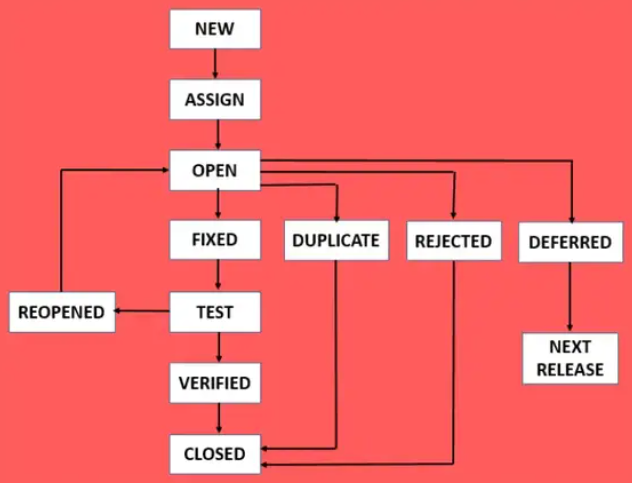
\includegraphics[width=0.6\textwidth]{bugLifecycle1.png}
            \attribution{https://www.softwaretestingmaterial.com/bug-life-cycle/}
        \end{center}
    \end{frame}

    \begin{frame}
        \frametitle{Ещё пример}
        \begin{center}
            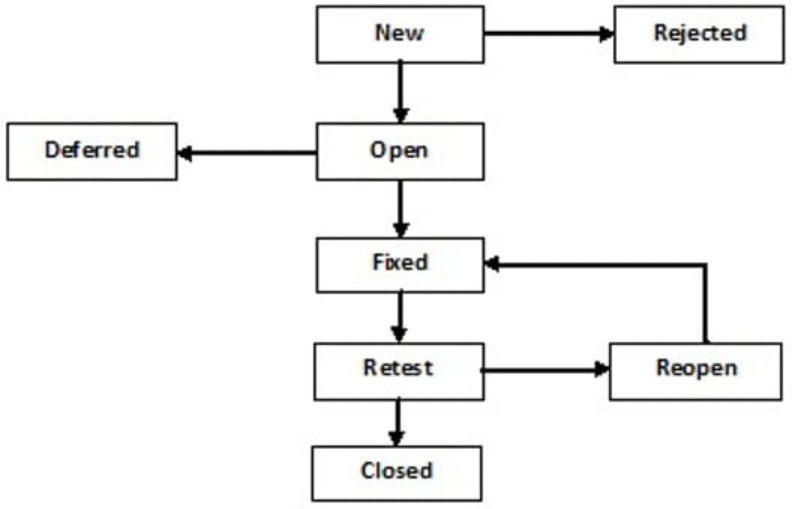
\includegraphics[width=0.6\textwidth]{bugLifecycle2.png}
            \attribution{https://www.softwaretestinghelp.com/bug-life-cycle/}
        \end{center}
    \end{frame}

    \begin{frame}
        \frametitle{Слишком простой пример}
        \begin{center}
            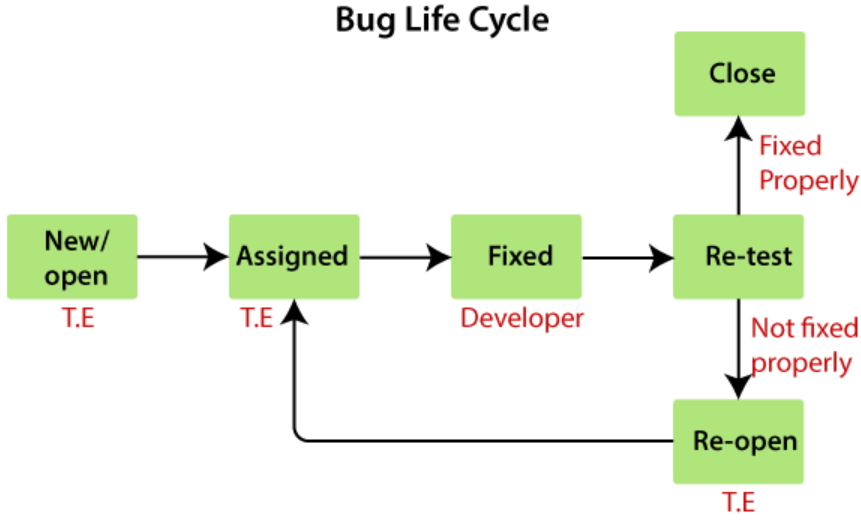
\includegraphics[width=0.6\textwidth]{bugLifecycle3.png}
            \attribution{https://www.javatpoint.com/software-testing-bug-life-cycle}
        \end{center}
    \end{frame}

    \begin{frame}
        \frametitle{Системы отслеживания ошибок}
        \begin{itemize}
            \item Jira
            \item GitHub Issues, Gitlab и т.п.
            \item Yandex Tracker
            \item Microsoft Team Foundation Server
            \item Redmine
            \item JetBrains Youtrack
            \item Bugzilla
            \item OpenProject
        \end{itemize}
    \end{frame}

\end{document}